\documentclass[11pt]{article}
% Preamble for "How a Proof Becomes a Program" — the LaTeX-source edition.
% Compiles with pdflatex (pure-ASCII source; all math via LaTeX commands).

\usepackage[T1]{fontenc}
\usepackage{textcomp}
\usepackage{amsmath}
\usepackage{amsthm}
\usepackage{mathtools}
\usepackage{newpxtext}                 % Palatino-family text (book-quality serif)
\usepackage{newpxmath}                 % matching math (provides \mathbb, etc.)
\usepackage[varqu,scaled=0.94]{zi4}    % Inconsolata monospace
\usepackage{microtype}

\usepackage[letterpaper,margin=1.15in]{geometry}
\usepackage{xcolor}
\usepackage{booktabs}
\usepackage{array}
\usepackage{enumitem}
\setlist{itemsep=3pt,topsep=5pt,parsep=0pt}

\usepackage{titlesec}
\titleformat{\section}{\normalfont\Large\bfseries\color{accent}}{}{0pt}{}
\titleformat{\subsection}{\normalfont\large\bfseries}{}{0pt}{}
\titlespacing*{\section}{0pt}{1.9\baselineskip}{0.8\baselineskip}
\titlespacing*{\subsection}{0pt}{1.2\baselineskip}{0.4\baselineskip}

\usepackage{tikz}
\usetikzlibrary{arrows.meta,positioning,calc,fit,backgrounds,chains,
  shapes.geometric,shapes.misc,decorations.pathreplacing}
\usepackage{caption}
\captionsetup{font=small,labelfont={bf,color=accent},skip=6pt}

\usepackage[numbers,sort&compress]{natbib}
\usepackage[hidelinks]{hyperref}

% ---------- palette ----------
\definecolor{accent}{HTML}{1A5276}   % deep blue  (structure)
\definecolor{amber}{HTML}{B9770E}    % amber      (the "live" value)
\definecolor{good}{HTML}{1E8449}     % green      (choice-free / runs)
\definecolor{bad}{HTML}{922B21}      % red        (classical / does not run)
\definecolor{boxbg}{HTML}{F3F6F8}
\definecolor{boxbg2}{HTML}{FBF5EA}
\definecolor{rulec}{HTML}{9FB0BA}

% ---------- notation (\ensuremath so each works in text and math) ----------
\newcommand{\Nat}{\ensuremath{\mathbb{N}}}
\newcommand{\PT}{\mathsf{PureType}}          % math-only (subscripted)
\newcommand{\good}{\ensuremath{\operatorname{good}}}
\newcommand{\fib}{\ensuremath{\operatorname{fib}}}
\newcommand{\hydra}{\ensuremath{\operatorname{hydra}}}
\newcommand{\lev}{\ell}                       % math-only
\newcommand{\rz}{\ensuremath{\Vdash}}
\newcommand{\extract}{\ensuremath{\mathsf{extract}}}
\newcommand{\CtQ}{\ensuremath{\mathsf{CtQ}}}
\newcommand{\epsz}{\ensuremath{\varepsilon_0}}
\newcommand{\fst}{\pi_1}                       % math-only
\newcommand{\snd}{\pi_2}                       % math-only
\newcommand{\code}[1]{\texttt{#1}}

% a key statement, set off as an indented italic callout with an accent rule
\newenvironment{keystmt}{%
  \par\smallskip\noindent\begin{list}{}{%
    \setlength{\leftmargin}{1.6em}\setlength{\rightmargin}{1.2em}%
    \setlength{\topsep}{4pt}}\item[\textcolor{accent}{\rule[-0.2ex]{2.2pt}{1.2em}}]\itshape}%
  {\end{list}\smallskip}

% ---------- tikz styles ----------
\tikzset{
  box/.style={draw=accent,line width=0.7pt,rounded corners=2.5pt,fill=boxbg,
    inner sep=6pt,align=center,font=\small,minimum height=2.4em},
  boxa/.style={box,draw=amber,fill=boxbg2},
  boxg/.style={box,draw=good,fill=good!8},
  boxb/.style={box,draw=bad,fill=bad!7},
  plain/.style={inner sep=3pt,align=center,font=\small},
  flow/.style={-{Latex[length=2.4mm,width=1.8mm]},line width=0.8pt,draw=accent!85!black},
  flowa/.style={flow,draw=amber!85!black},
  ladder/.style={draw=rulec,line width=0.6pt,-{Latex[length=2mm]}},
  elabel/.style={font=\footnotesize\itshape,fill=white,inner sep=1.5pt,text=black!70},
  figcap/.style={font=\footnotesize,text=black!65,align=center},
  % --- descent-certificate motif (repeated across Act IV) ---
  dbox/.style={draw=accent,line width=0.6pt,rounded corners=2pt,fill=boxbg,
    inner sep=0pt,minimum width=8mm,minimum height=6.5mm,font=\footnotesize,align=center},
  dzero/.style={dbox,draw=good,fill=good!12},          % the certificate hits bottom
  dup/.style={dbox,draw=amber,fill=boxbg2},            % the visible quantity, climbing
  dlab/.style={font=\footnotesize\itshape,text=accent},% "descent certificate: ..."
}

\geometry{margin=0.9in}
\pagestyle{empty}

\begin{document}
\begin{center}
  {\LARGE\bfseries\color{accent} One construction, two readings}\\[2pt]
  {\itshape the proof \emph{is} the program --- extraction is the map that shows it}
\end{center}
\vspace{2pt}

\noindent
Modified realizability is the Curry--Howard correspondence with the map made
explicit: a proof (a \code{Deriv}) and its extracted program (a realizer) are
distinct objects joined by \extract, and \extract\ is \emph{structure-preserving}
--- it sends each proof rule to one program operation. The dictionary, and then
the same dictionary at work on two theorems.

\vspace{6pt}
\begin{center}
\renewcommand{\arraystretch}{1.18}
\small
\begin{tabular}{@{}ll l@{}}
\toprule
\textbf{Proposition / proof rule} & \textbf{Program operation} & \textbf{as a type} \\
\midrule
$\forall$-intro / $\forall$-elim & $\lambda k.\,\_$ \ / \ apply at a value & $\Pi$ (dependent function)\\
$\rightarrow$-intro / $\rightarrow$-elim & $\lambda h.\,\_$ \ / \ apply & function \\
$\exists$-intro / $\exists$-elim & \code{return}$\ \langle w,\,\cdot\rangle$ \ / \ \code{let}$\ \langle w,p\rangle$ & $\Sigma$ (dependent pair) \\
$\land$-intro / $\lor$-elim & pair $\langle\_,\_\rangle$ \ / \ \code{case} & product / sum \\
induction & fold-recursion & $\mathsf{Nat.rec}$ \\
transfinite induction $\mathrm{TI}(\epsz)$ & well-founded recursion along $\prec$ & $\mathsf{WellFounded.fix}$ \\
hypothesis / induction hyp. & variable \ / \ \emph{recursive call} & bound variable \\
equation, $\bot$ & $\cdot$ \ (erased --- no runtime content) & proof-irrelevant \\
\bottomrule
\end{tabular}
\end{center}

\vspace{10pt}
\noindent{\bfseries\color{accent} Reading 1 --- witness supplied by hand $\Rightarrow$ a constant.}
\ \ The proof of $\exists s.\ \good(3,s)=0$ \emph{contains} the answer; extraction reads it out.

\begin{center}
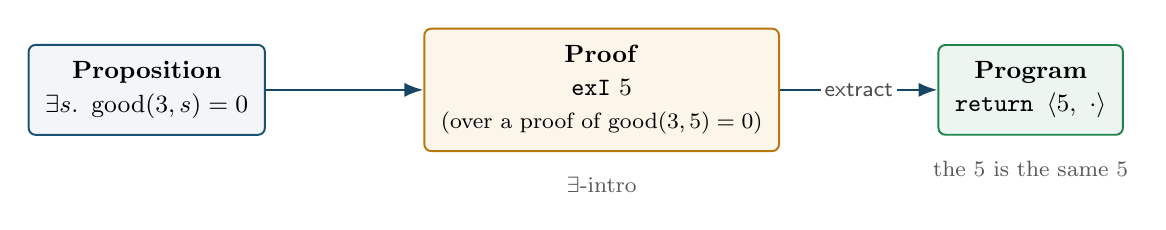
\begin{tikzpicture}[node distance=10mm and 20mm]
  \node[box,align=center](prop){\textbf{Proposition}\\[1pt]$\exists s.\ \good(3,s)=0$};
  \node[boxa,align=center,right=of prop](proof){\textbf{Proof}\\[1pt]\code{exI}~$5$\\[1pt]\footnotesize (over a proof of $\good(3,5)=0$)};
  \node[boxg,align=center,right=of proof](prog){\textbf{Program}\\[1pt]\code{return }$\langle 5,\ \cdot\rangle$};
  \draw[flow](prop)--(proof);
  \draw[flow](proof)--node[elabel]{\extract}(prog);
  \node[figcap,below=2mm of proof]{$\exists$-intro};
  \node[figcap,below=2mm of prog]{the $5$ is the same $5$};
\end{tikzpicture}
\end{center}

\vspace{6pt}
\noindent{\bfseries\color{accent} Reading 2 --- witness produced by $\mathrm{TI}(\epsz)$ $\Rightarrow$ a recursion.}
\ \ The proof of $\forall m\,\exists s.\ \good(m,s)=0$ contains no literal witness ---
it contains a \emph{recursion}, and extraction turns the recursion into a program
that \emph{computes} the stopping step. Left, the proof; right, the extracted
program; each row is one rule of the dictionary. (This is the exact output of
\code{\#realizerCH goodsteinTheorem}, abbreviated to the spine.)

\vspace{4pt}
\begin{center}
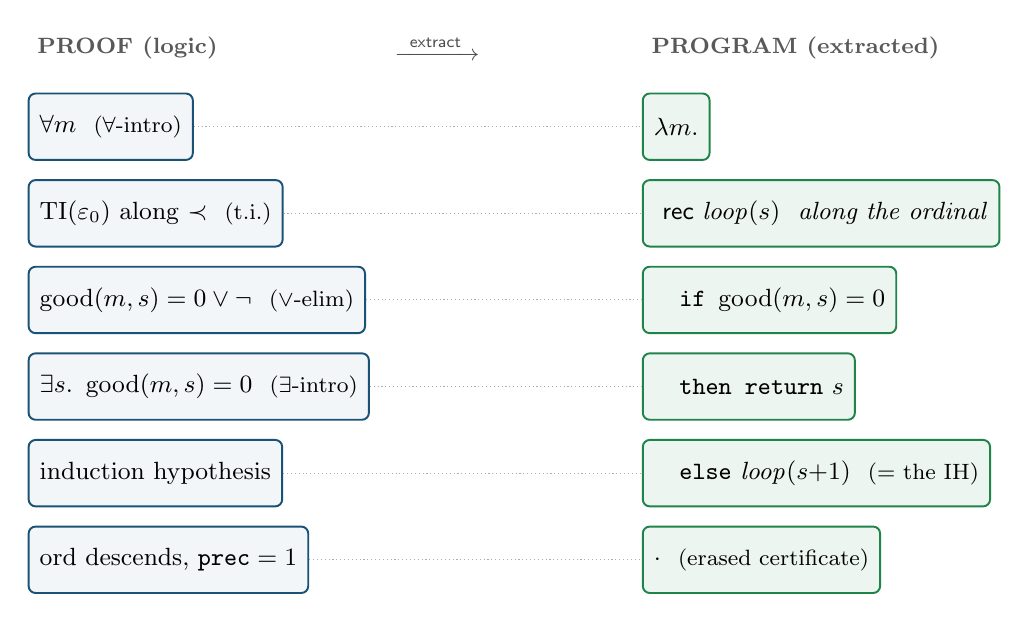
\begin{tikzpicture}[
   L/.style={box,anchor=west,align=left,inner sep=4pt,font=\small},
   R/.style={boxg,anchor=west,align=left,inner sep=4pt,font=\small}]
  % column headers
  \node[figcap,anchor=west,font=\footnotesize\bfseries] at (0,10mm){PROOF (logic)};
  \node[figcap,anchor=west,font=\footnotesize\bfseries] at (78mm,10mm){PROGRAM (extracted)};
  \node[elabel] at (52mm,10mm){$\xrightarrow{\ \extract\ }$};
  % logic column (left, x = 0) and program column (right, x = 78mm), aligned by y
  \node[L,anchor=west] (l1) at (0,  0mm){$\forall m$ \ \footnotesize($\forall$-intro)};
  \node[L,anchor=west] (l2) at (0,-11mm){$\mathrm{TI}(\epsz)$ along $\prec$ \ \footnotesize(t.i.)};
  \node[L,anchor=west] (l3) at (0,-22mm){$\good(m,s)=0 \lor \neg$ \ \footnotesize($\lor$-elim)};
  \node[L,anchor=west] (l4) at (0,-33mm){$\exists s.\ \good(m,s)=0$ \ \footnotesize($\exists$-intro)};
  \node[L,anchor=west] (l5) at (0,-44mm){induction hypothesis};
  \node[L,anchor=west] (l6) at (0,-55mm){$\mathrm{ord}$ descends, $\code{prec}=1$};
  \node[R,anchor=west] (r1) at (78mm,  0mm){$\lambda m.$};
  \node[R,anchor=west] (r2) at (78mm,-11mm){$\ \mathsf{rec}\ \mathit{loop}(s)$ \emph{ along the ordinal}};
  \node[R,anchor=west] (r3) at (78mm,-22mm){$\ \ \ \code{if}\ \good(m,s)=0$};
  \node[R,anchor=west] (r4) at (78mm,-33mm){$\ \ \ \code{then return}\ s$};
  \node[R,anchor=west] (r5) at (78mm,-44mm){$\ \ \ \code{else}\ \mathit{loop}(s{+}1)$ \ \footnotesize(= the IH)};
  \node[R,anchor=west] (r6) at (78mm,-55mm){$\cdot$ \ \footnotesize(erased certificate)};
  \foreach \i in {1,2,3,4,5,6}
    \draw[densely dotted,rulec] (l\i.east) -- (r\i.west);
\end{tikzpicture}
\end{center}

\vspace{2pt}
\begin{center}\itshape\small
The same 29-node object is a proof that every Goodstein sequence terminates
(\code{\#print goodsteinTheorem}) and a program that computes when
(\code{\#realizer goodsteinTheorem}). The shape of the induction is the shape of
the recursion: witness-by-hand gives a constant, witness-by-$\mathrm{TI}(\epsz)$
gives an $\epsz$-recursion. The induction hypothesis \emph{is} the recursive
call; the ordinal descent is the one part with no runtime content.
\end{center}

\end{document}
